% DHL's Design notes:


% Motifs:

% gadgets are a set of general algorithms that implement control-flow patterns
% in a decentralized manner and can execute on constituent functions alongside
% user code.

% gadgets are platform-independent control-flow patterns that can be implemented
% efficiently in a decentralized manner.

% Control-flow patterns.

% IR describes control-flow "logic"



% %%%%% Notes


% Graphs:

% A graph that constrasts application \emph{execution} with \name{} and
% centralized orchestrator. It's ok for the application to be artificial but it
% should sufficient complex with chain, fan-out and fan-in. The orchestrator
% figure should show the orchestrator centralizing control flow and driving the
% execution. The \name{} graph should show functions with gadgets and zoom in,
% similar to Figure 2(c), to show the runtime wrapper and interactions with the
% data store. The centralized orhcestrator should have the same color with the
% gadgets. Different from the current (a), ingress should show gadgets too.

% A graph that show the compilation stage. It's important to show what we gain
% at compile time: assigning gadgets to nodes in the directed graph.

% Architecture%%%%%%%%%%%%%%%

% no new component. Instead, 

% a set of general algorithms, called ``gadgets'', that  implements control-flow
% patterns in a decentralized way using basic serverless APIs, 

% Similar to existing systems, \name{} takes the user write workflows in the
% form of a directed graph. Instead of an centralized orchestrator executing the
% graph, \name{} ... Figure~\ref{fig:arch:centralized} and \ref{fig:arch} constrasts.



% Computations are a direct graph.


% Describe the abstract machine (the serverless abstraction with async invoke +
% strongly consistent data store with conditional updates) and here in this
% section.

% "strongly consistent data store with conditional updates". Is this going to
% raise eyebrows when we mention S3? Because technically, S3 does not have a
% conditional update API. We implement it with its object versions feature,
% which has to be turned on when creating the bucket.



% Gadgets%%%%%%%%%%%%%%%%%

% Gadgets are the general algorithms that implements control-flow patterns in a
% decentralized way against a basic serverless abstraction that is universially
% supported by all serverless providers.

% A set of general algorithms that implements control-flow patterns in a
% decentralized way using basic serverless APIs.


% Different from ad-hoc compositions: 1. use of data store 2.
% Control flow logic not only on the caller but also on the callee 3. standard,
% off-the-shelf primitives that's not application specific that developers build
% from scratch.


% Then use the gadget section to describe the algorithm for each pattern.

% State that "\name{} provides four gadgets that map can express a rich variety
% of workflows efficiently, including a superset of workflows expressible in
% Step Functions". Keep the example applications for each pattern that's
% currently in the text to show the usefulness and necessity for each pattern.

% supports all commonly found patterns. In SF, and in DAGs.

% unum IR%%%%%%%%%%%%%

% intermediate representation language that encodes control-flow 

% The IR language primary encodes gadgets but also provides other programmable
% constructs that enables dynamic behavior at runtime. Have a table of
% programmable constructs? (Conditional, \$ret, \$0, \$size)

% In pratice the IR is a set of JSON file, one for each edge in the control flow
% graph transition from a function to the next in the control-flow.

% Each function node has a unique name.

% Scalar, Map, Parallel are pretty straightforward because it dosen't have data
% dependency on other functions in the workflow.

% Fan-in expresses data dependencies. More flexible than Step Functions because
% SF only supports dependencies within a state. unum fan-in can specify any
% function in the workflow.

% Programmable constructs: 

% Conditional: branch, termination condition for a loop, foward condition for a
% selective set of parallel branches



% Frontend compiler%%%%%%%%%%%%%%%%

% how to assign gadgets

% Runtime%%%%%%%%%%%%

% XXX: Transparently wraps around user code and interposes on entry and exit -> keep user code unchanged



% Show the runtime input payload structure


% Execution guarantees%%%%%%%%%%%%%%%%%%

% XXX: All unum runtime code needs to be idempotent

\section{System Architecture}\label{sec:architecture}

\begin{figure*}[t]
    \centering
    \begin{subfigure}[t]{0.8\textwidth}
        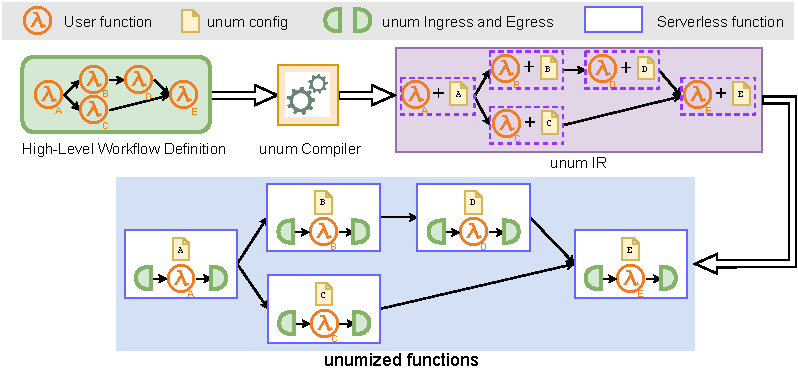
\includegraphics[width=\columnwidth]{figures/unum-arch-compile-time.pdf}
        \caption{Stateful serverless computations form a directed graph. Nodes
                are user defined FaaS functions and workflow ``gadgets'' that dictate the
                communication pattern between user functions.}
        \label{fig:arch:unum-compile-time}
        % unum injects gadgets to functions at compile time. But more
        % specifically, unum injects an encoding of gadgets at compile time.
        % The encoding expresses control-flow transitions just like what the
        % high-level workflow definition.
    \end{subfigure}
    \begin{subfigure}[b]{\columnwidth}
    \centering
        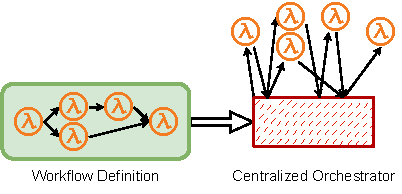
\includegraphics[width=0.8\columnwidth]{figures/unum-arch-centralized.pdf}
        \caption{A typical stateful serverless system drives workflow logic
                 using a centralized controller that manages the computation's state-machine.}
        \label{fig:arch:centralized}
    \end{subfigure}
    \hfill
    \begin{subfigure}[b]{\columnwidth}
    \centering
        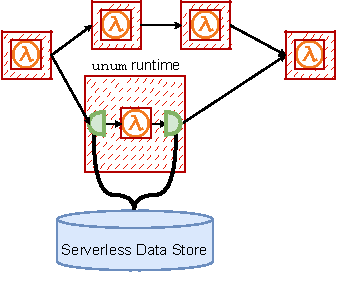
\includegraphics[width=0.5\columnwidth]{figures/unum-arch-runtime.pdf}
        \caption{\name{} decentralizes controller logic by running local state
                 transitions alongside Faas functions inside the \name{} runtime
                library. There is no centralized controller, instead \name{} relies on existing
                serverless datastores such as DynamoDB or Cosmos DB.}
        \label{fig:arch:unum-runtime}
    \end{subfigure}
    \caption{\name{} System Overview. Serverless computations form a directed
            graph that encode sequential and data dependencies between functions. Workflow
            orchestrators drive these graphs by centralizing control flow logic and
            interposing on all communication between functions. \name{},
            instead, decentralizes control flow logic among the functions with
            no need for a separate orchestration system.}
    \label{fig:arch}
\end{figure*}

\dhl{TODO: Explain the purpose and use of the data store early on in the
design portion of the paper. Probably also a good idea to motivate the use of
data store in the background section.}


A key design feature of \name{} is to not introduce new components to the
basic serverless infrastructure. Instead, \name{} invents a set of general
algorithms, called ``gadgets'', that implement control-flow patterns in a
decentralized manner and can execute on constituent functions alongside user
code. Additionally, \name{} encompasses an intermediate representation
language that encodes gadgets and describes control-flow logic, a frontend
compiler that transforms higher-level workflow representations written by
developers to the intermediate representation, and a runtime library that
implements the gadgets with platform-specific APIs.

Similar to existing systems~\cite{aws-step-functions, google-workflows,
google-cloud-composer, gg-atc}, \name{} users define workflows using
high-level description languages, such as AWS Step Functions, that express the
control-flow in the form of directed graphs where nodes are serverless
functions and edges are control-flow transitions between functions. A
transition from function \texttt{F} to \texttt{G} involves (1). invoking an
instance of \texttt{G} and (2). passing \texttt{F}'s result to the \texttt{G}
instance.
\dhl{Describing the directed graph abstraction helps clarify and set the
mental model. Should also explain from the directed graph perspective in the
background:workflow orchestrators section so that this is not the first time
we say this. State machines (i.e., Step Functions) and DAGs (i.e., Google
Workflows, Apache Airflow, Dask) all fit into direct graphs.}

But different from existing systems where a centralized orchestrator executes
control-flow graphs by invoking every function and receiving their results
(Figure~\ref{fig:arch:centralized}), \name{} transforms this high-level
description to \name{}'s intermediate representation (IR) and embeds portions
of the control-flow logic to appropriate functions, \emph{at compile time}
(Figure~\ref{fig:arch:unum-compile-time}). Control-flow in the IR is encoded
as ``gadgets''---platform-independent control-flow patterns that can be
implemented efficiently in a decentralized manner. Finally, developers combine
their functions with a platform-specific \name{} runtime which implements
gadgets using platform-specific APIs and datastores.

During execution, the \name{} runtime performs control-flow transitions by
running its assigned gadget (Figure~\ref{fig:arch:unum-runtime}). The runtime
transparently interposes on user code entry and exit. On entry, the runtime
reads data sent by the caller and passes it to user code. On exit, the runtime
gets user code result and invokes the next function with it. Additionally, the
runtime implements a checkpointing mechanism that ensures exactly-once
semantics.

\dhl{say more about exactly-once semantics here?}


\amit{TODO: gadgets are the secret sauce, in particular noticing that fan-in needs to
be split between the source and target functions \emph{and} that source
functions must coordinate.}
\amit{TODO: gadgets don't run where programmers express them. Example with
fan-in. This is kind of the ``magic'' of the front-end compiler.}
\dhl{I'm not sure the above 2 statements are true. Maybe because I didn't
understand your "move" gadgets mental model and it can work. Let's chat.}



\section{Gadgets}\label{sec:gadgets}

A key challenge in decentralizing control-flow is determining where to store
control-flow state and where to execute transitions. \name{} uses the notion
of gadgets---a set of general algorithms for control-flow patterns that can be
implemented efficiently in a decentralized manner. At compile-time,
\name{} derives the necessary gadgets from a workflow definition written in
high-level description language and attaches them to the approprite user
functions. The \name{} runtime that wraps the user function implements the
gadgets with platform-specific APIs and executes its assigned gadget during
execution.

Logically, gadgets are treated as a special kind of node in the control-flow
graph and placed alongside user function nodes. Each gadget is implemented as
a pair of nodes: an ingress node and an egress node. Every user function in
\name{} has exactly one input edge coming from an ingress node and one output
edge going to an egress node, i.e., the user function is invoked once with a
single value by an ingress node and outputs its result to a single egress
node. When placing a gadget in the graph, the egress node is appended to the
upstream function and the matching ingress node is prepended to the immediate
downstream node along an existing edge.

\name{} provides four gadgets that can express a rich variety of workflows
efficiently, including a superset of workflows expressible in AWS Step
Functions. Table~\ref{tab:gadgets} lists the gadgets available in \name{} and
we explain each in detail in this section.

\name{} gadgets are designed against a basic serverless abstraction that is
universally supported by current platforms. The algorithms themselves are
platform-agnostic and use only basic serverless APIs. Specifically, they rely
on an asynchronous invocation API for FaaS functions and a strongly consistent
data store that supports conditional writes.

\dhl{"strongly consistent data store with conditional writes". Is this going
to raise eyebrows when we later mention S3? Because technically, S3 does not
have a conditional write API. We implement it with its object versions
feature, which has to be turned on when creating the bucket. Maybe better to
call it something else.}

% \dhl{I'm not sure it makes sense to treate fan-in specially on the directed
% graph level. In the previous version, the ingress gadget node on the fan-in
% doesn't really perform any \emph{control-flow logic}. It just reads the input
% data. And this is the same behavior across all gadgets. The ingress just read
% data, whether from a HTTP packet or from DynamoDB. You can pass a vector of
% pointers via a chain gadget and the ingress will do the same thing. But I
% guess more importantly, the ingress is simply and uniform enough that treating
% fan-in specially in our explanation doesn't add much value.}

\dhl{From previous version: "At compile-time, \name{} injects these gadgets
into the nearest function and executes them in the \name{} runtime that wraps
the function. Thus there is no system overhead for running the gadgets---they
are, effectively, embedded in the functions themselves."The last sentence is
unclear to me. Running gadgets incur latency and additional Lambda billing.}



\begin{table}[t!]
  \centering
  \begin{tabular}{ |m{8em}| m{13em} | }
    \hline
      \texttt{chain(a,b) }& Invokes function \texttt{b} with the output of \texttt{a} \\
    \hline
      \texttt{fanOut(a, [b])} & Invokes each element of \texttt{[b]} with the output from \texttt{a} \\
    \hline
      \texttt{map(a, b)} & Invokes \texttt{b} once for each element in the vector output of \texttt{a} \\
    \hline
      \texttt{fanIn([a], b)} & Invokes \texttt{b} once with the vector of outputs from each of \texttt{[a]} \\
    \hline
\end{tabular}
  \caption{\name{} workflows express complex interactions using a small set of
  gadgets. \texttt{a} and \texttt{b} are names that identify specific function
  instances in the control flow graph.}
  \label{tab:gadgets}
\end{table}

\dhl{pseudocode for each gadget? or a simple schematics showing the pattern
graphically?}

\paragraph{Chain}
Chaining is a simple but common control-flow pattern. For example, an
application might include a function (the source) that processes input data
from a sensor followed by another function (the target) that adjusts an
actuator based on the processed input. The \texttt{chain} gadget connects two
user functions together by invoking the target with the result of the source.
It consists of one egress node and one ingress node. The egress node is
appended to the source function while the ingress is prepended to the target.

At runtime, the egress node runs on the same FaaS function as the source and
ingress as the target. The egress gets the output of the source user function
and uses the platform's asynchronous function invocation API to call the
target function directly from the source. The ingress on the target reads the
data sent from source and passes it to the target user function. Depending on
the platform's implementation of asynchronous invoke API, the ingress might
read the input data from a data store or the received HTTP message.


\paragraph{Fan-out}
Another common interaction processes the output of a function in different
ways in parallel. For example, an social network application might perform
several independent functions given a new user post, such as URL shortening
and resolving other users mentioned in the post. The \texttt{fanOut} gadget
invokes a vector of functions (branches) each with the output of the same
source function. The gadget consists of one egress node and many ingress
nodes. Similar to chaining, the egress node is appended to and runs with the
source function and it uses the asynchronous invocation API to invoke each
branch. But in this case, an ingress node is prepended to each branch and
reads the input data sent from the source and passes it to its user function.

\paragraph{Map}
An application may also perform the same function on multiple outputs of a
source function. For example, a photo management application might unpack an
archive of high-resolution images in one function and perform compression on
each of the resulting images. The \texttt{map} gadget invokes the same
function once for each element in a vector of outputs from the source
function. The algorithm and placement of \texttt{map} ingress and egress nodes
are identical to \texttt{fanOut}.

\amit{TODO: Are there special considerations for exactly-once
semantics? i.e. is checkpointing different than it is in chaining?}
\dhl{No. In fact checkpoint works independently from the control-flow
patterns. The algorithm for exactly-once semantics is the same across all
gadgets.

Now specifically for fan-out it works like this: the fan-out initiator node
will checkpoint right after user code returns which saves the data that is
about to be fanned out. After checkpointing completes, the fan-out initiator
node invokes the branches. If it crashes at any point during the series of
invocations, unum retries the fan-out initiator lambda. The unum runtime on
the lambda will see that a checkpoint with its name already exists, and
therefore skips running the user function. But it will not skip retrying the
fan-out, and it restarts the fan-out \emph{from the beginning}, which will
result in duplicate instances for some or even all of the branches. But that
is OK. Because the unum runtime protects against duplicates and still ensures
exactly-once semantics. If the duplicates are concurrent (i.e., the original
branch instances are still running), we protects that with a conditional write
when checkpointing the results so only one instance of the duplicates will
win. If the duplicates are nonconcurrent (i.e., the original branch instances
already completed), the duplicates will skip running the user functions
altogether.

The fan-out initiator will keep retrying until a full fan-out is performed to
make sure at-least-once invocation.

% (explaining this makes me appreciate the consistency papers even more, 'cuz
% this stuff is hard to explain.)

So the patterns do not change the algorithms with which we provide exactly
once. They work independently from each other. The only real gotcha we need to
be careful with in \emph{implementing} exactly-once is nonidempotent
operations, as pointed out by you. Specifically, the synchronizations across
branches have to be idempotent. The purpose is prevent pre-mature fan-in.

Given the complexity of the exactly-once algorithm and the fact that it works
independently from gadgets, I think it works better if we have separate
section just for the execution guarantee and do not explain the details in
this section.}

\amit{TODO: I feel like there is a bunch of complexity, particularly with
fan-in, do with assigning indexes to branches, etc, that is part of the
platform-agnostic design of unum, so should be here. But I don't recall the
specifics. Are there also similar things for the other gadgets?}
\dhl{I'm not sure what you mean by "similar things". But the branch indexes
are assigned by the fan-\emph{out} node. The purpose is to give each node in
the graph a unique name. I really don't think we should discuss the naming
aspect in this section. I think this structure of writing the design works
very well if we keep the gadgets to be general algorithms for control-flow
patterns that are designed against an abstract serverless machine. We can talk
about what we require from the serverless abstraction, but we shouldn't talk
about the naming scheme. The gadget just cares that each function has a name,
that you can identify them. It does not care how. Then in the IR section, we
can talk about how the IR actually encodes the gadgets, and that's where we
can explain that (1). we need each function to have a unique name for fan-in
to work because we need to clearly identify which node's result to fan-in
from, and we can have multiple instances of the same function in the graph
because of fan-in and map. (2). our naming scheme is to assign an integer,
starting with 0 and incrementing monotonically by 1, to each branch. And
that's it. That's all the information we need at the IR level. And finally in
the runtime section, we show the input payload which has a field for the
branch index, and that's how we actually implement this piece of information.
And we explain that the fan-out node adds this field to the payload when
invoking each branch. It's like the storage layers where each layer adds a bit
more information to enable specific additional functionalities.}

\paragraph{Fan-in}

After processing data with many parallel branches, applications commonly want
to aggregate results. For example, a video encoder might divide a large video
into chunks, encode each in parallel and then concatenant all the encoded
chunks together. The \texttt{fanIn} gadget takes the outputs from a vector of
functions (the fan-in branches) and invokes a single ``sink'' function. The
\texttt{fanIn} gadget consists of one ingress node and many egress nodes. Each
fan-in branch is appended an egress node and the sink function is prepended
the only ingress node.

% TBD
%
% The \texttt{fanIn} gadget gadget ensures that the control-flow transition is
% \emph{wait-free} and that the sink function is invoked only once.
% Specifically, its semantics is that the sink function is invoked only once
% when all upstream functions in the vector have completed.

% To realize the semantics, the \texttt{fanIn} gadget has to solve several
% challenges. Access to branches data. wait-free. and synchronize.

The \texttt{fanIn} gadget ensures that the control-flow transition is
\emph{wait-free}. That is the sink function is invoked only when all upstream
functions in the vector have completed so that the sink function does have to
be spun up ahead of time and waste CPU cycles (and therefore extra billing)
idly waiting for upstream functions to finish. Moreover, the upstream
functions in \texttt{fanIn} simply terminates when done and do not wait for
each other either.

To achieve this, the \texttt{fanIn} egress always writes the output of its
user function to a data store. This serves two purposes: (1). it allows any of
the upstream functions to access the output of other upstream functions (2).
it signals the completion of a function. This way, each egress can simply
writes its output and terminate. Other egress nodes can still access completed
egress' data after they terminate. Any one of the egress can invoke the sink
function. And any one of the egress can see if other egress has completed or
not. \dhl{definitely needs better phrasing but hopeful the point makes sense}

Strongly consistent data store is important here because it prevents the
scenarios where all egress have written outputs but none of them sees that all
have completed, which results in the sink function never invoked.

Additionally, \texttt{fanIn} makes sure that when the sink function is
invoked, it is invoked only once. \name{} achieves this by having the egress
nodes synchronize with each other via the same data store such that only the
last-to-finish egress invokes the sink function. Synchronization is done with
atomic read-after-write over a single object. Specific implementation depends
on the data store and we discuss the details in \S\ref{sec:impl}. But all we
need is strong consistency with conditional writes.

The last-to-finish egress invokes the sink function with a vector of pointers
to each upstream function's stored output. The pointers are the in same order
as the vector of upstream function names. The ingress on the sink function
dereferences each point by reading from the data store and passes a vector of
output values to its user function.

Fan-in is a critical control-flow pattern to support and distinguishes \name{}
from ad-hoc trigger-based composition. \dhl{Do we want to constrast here? and
what should we say? Different from ad-hoc compositions: 1. use of data store
2. Control flow logic not only on the caller but also on the callee 3.
standard, off-the-shelf primitives that's not application specific that
developers build from scratch.}


\dhl{Propose name change for gadget -> nexus}

% chain = invoke, fan-out = a bunch of invoke, one for each continuation;
% Additionally, in the case of Map, one invoke for each element of the array
% (output of the user function).  fan-in .... well.... let's see. The semantics
% is: invoke the fan-in function once when all of its inputs are ready. In
% practice, it is each branch synchronize over the data store to see if all
% branches have completed. The last branch to complete calls invoke on the fan-in
% function, and pass it pointers to all branches results/checkpoints in the data
% store. The fan-in function first reads the branches' results, in order, via the
% pointers, then pass them as input to the user code.

\section{\name~IR}\label{sec:ir}

exporess control-flow logic. To express control-flow logic the IR first given
each function instance a unique name.

The naming scheme needs to encompass dynamic patterns such a map.

\begin{itemize}

    \item intermediate representation language that primarily encodes gadgets

    \item In practice, the \name{} IR is a set of configuration files (by default named
    \texttt{unum\_config.json}), one for each function node in the workflow.
    Every function has a \texttt{unum\_config.json} file deployed with it.

    \item Gadgets are encoded in the \texttt{"Next"} field. Give example for
    each gadget with code snippets. Explain the \texttt{"Name"} and
    \texttt{"InputType"} field.

    \item With the fan-in gadget, and the \texttt{"Values"} field, explain the
    need for IR to give each function node a unique name. The naming scheme
    works for dynamic patterns such as \texttt{map} where the number of
    branches is unknown at compile time. Explain the naming scheme.

    \item Fan-in expresses data dependencies. More flexible/expressive than
    Step Functions because SF only supports dependencies within a state. unum
    fan-in can specify any function in the workflow.

    \item The IR language primarily encodes gadgets but also provides other programmable
    constructs that enables dynamic behavior at runtime. For example
    Conditional: branch, termination condition for a loop, foward condition
    for a selective set of parallel branches. Value names in fan-in can
    include glob patterns to support fan-in of varying size. unum expands glob
    patterns during runtime. "Next Payload Modifiers" with runtime variables.
    Have a table of programmable constructs? (Conditional, \$ret, \$0, \$size)

\end{itemize}




\section{Runtime}

\begin{itemize}

    \item (focus on how gadgets are implemented and leave execution guarantee
    to its own section)

    \item \name{}'s runtime transparently interposes on user code's entry and
    exit such that developers do not change how they write application code at all.

    \item \name{} runtime implements all gadgets. And execute the assigned
    gadgets and control-flow logics based on the assigned IR file.

    \item Runtime has a particular input format in JSON.
    Figure~\ref{fig:input-format} shows the input format.

    \item \texttt{"Data"} field contains the input data to the user code. If
    the data is directly sent in the function invocation via HTTP (i.e.,
    \texttt{"Source": "http"}), the value of the "Value" field is passed to
    user code unchanged. If the \texttt{"Source"} field shows that the data is
    in the intermediary data store (e.g., \texttt{"Source": "dynamodb"}),
    \name{} reads the data from the data store and then pass it to user code.

    \item In practice, \name{} only passes data via the data store in the case
    of fan-in where results of multiple functions are needed. In that case,
    the \texttt{"Value"} field is an array of names of function checkpoints.
    \name{} reads each checkpoint in the array in order and passes the data as
    an array to user code.

    \item \texttt{"Session"} field contains a UUID string that uniquely
    identifies a workflow invocation. \name{} runtime on the entry function
    creates the UUID string when the function is invoked. The string
    propagates to all downstreams function instances that are part of the
    workflow invocation. Entry function can be any function on the graph. You
    can start with any function on the graph and invoke only a subsection. As
    long as the \texttt{"Session"} does not exist, \name{} runtime will create
    one.

    \item Checkpoint names are prefixed with the \texttt{"Session"} UUID
    string so that instances of the same function from different invocations
    do not overwrite each others' results.

    \item "Fan-out" field are part of fan-out functions' input payload.
    \name{} assigns each fan-out function an index.

    \item \name{} supports nested fan-outs with the \texttt{"OuterLoop"} field
    that is recursive.

    \item The "Index" in the "Fan-out" implements the branch name of the
    naming scheme in
    \S\ref{sec:ir}.

\end{itemize}

\section{Execution Guarantees}

Challenges to providing strong execution guarantees:

\begin{enumerate}

    \item Functions in the workflow can fail at any point.

    \item FaaS engines only provide at-least-once execution guarantee on
    individual functions. Triggering a function once might result in duplicate
    executions.

\end{enumerate}

Given the limitation of the underlying FaaS engines, \name{} cannot guarantee
exactly-once execution on \emph{individual functions}. However, \name{}
guarantees:

\begin{enumerate}

    \item At-least-once invocation on individual functions. This ensures that a
    workflow invocation will not just stuck somewhere and not proceed.

    \item In a particular workflow invocation, a particular function will
    always be invoked with the exact same input.

    \item Each workflow invocation will produce exactly one result. Even if
    there happen to be duplicate executions of functions, and even if the
    functions are non-deterministic, only a single result is recorded, while
    any duplicate and potentially diverging results are discarded.

\end{enumerate}

When a workflow execution crashes before finishing, \name{} only retries the
function where the crash happens instead of restarting the entire workflow.
\name{} leverages the automatic retry feature that most FaaS engines already provide
for individual functions~\cite{azure-functions-retry,
google-cloud-functions-retry, aws-lambda-async-invoke}.

\name{} checkpointing process is the following:

First, before running user code, the ingress checks to see if a checkpoint
already exists for the invocation. If it does, \name{} skips running user code
and uses the checkpoint's content as the result. The egress will invoke the
continuation again in case the prior execution crashed after checkpointing but
before running the continuation. This makes sure that if a step in the
workflow has completed and persisted, it will not run again.

If a checkpoint doesn't exist, unum runs the user code. After the user
function completes, unum checkpoints the result into the data store and runs
the continuation.


\section{Old Design}\label{sec:design}

% Notes(alevy):
%
% * Consider splitting design section into separate sections for System Architecture and IR/Language
% * Design needs to describe the (non)-architecture of unum. There are pieces of functionality that typically exist in a controller that still exist in unum, they are just embedded in
% unum runtime. Maybe we can give this 'component' a name, like a distributed controller (the unum runtime then implements the distributed controller).
% * The design includes too many implementation specific details, and doesn't really describe the high level operations. If the big question is 'how do you implement fan-out / fan-in
%   in a distributed way?', the section should answer that directly (same for other interactions which are much simpler).
% * Similarly, we need to describe the interactions that unum provides and sort of hand-wave argue that these are the right set of interactions (perhaps by pseudo-code example).
%
% Terms to use:
% * 'Gadgets': The interactions that are encoded in unum_config (fan-out, fan-in, chain, etc)
% * 'Execution graph': where nodes are either user-code (Lambda functions) or gadgets, edges exiting user-code always enter gadgets. Instead of talking about
%    continuations (I really don't think that Unum has something that looks like continuations), this execution graph is the IR and the runtime reifies the
%    execution graph by embedding gadgets in lambdas themselves.

%\begin{figure*}[t]
%    \centering
%    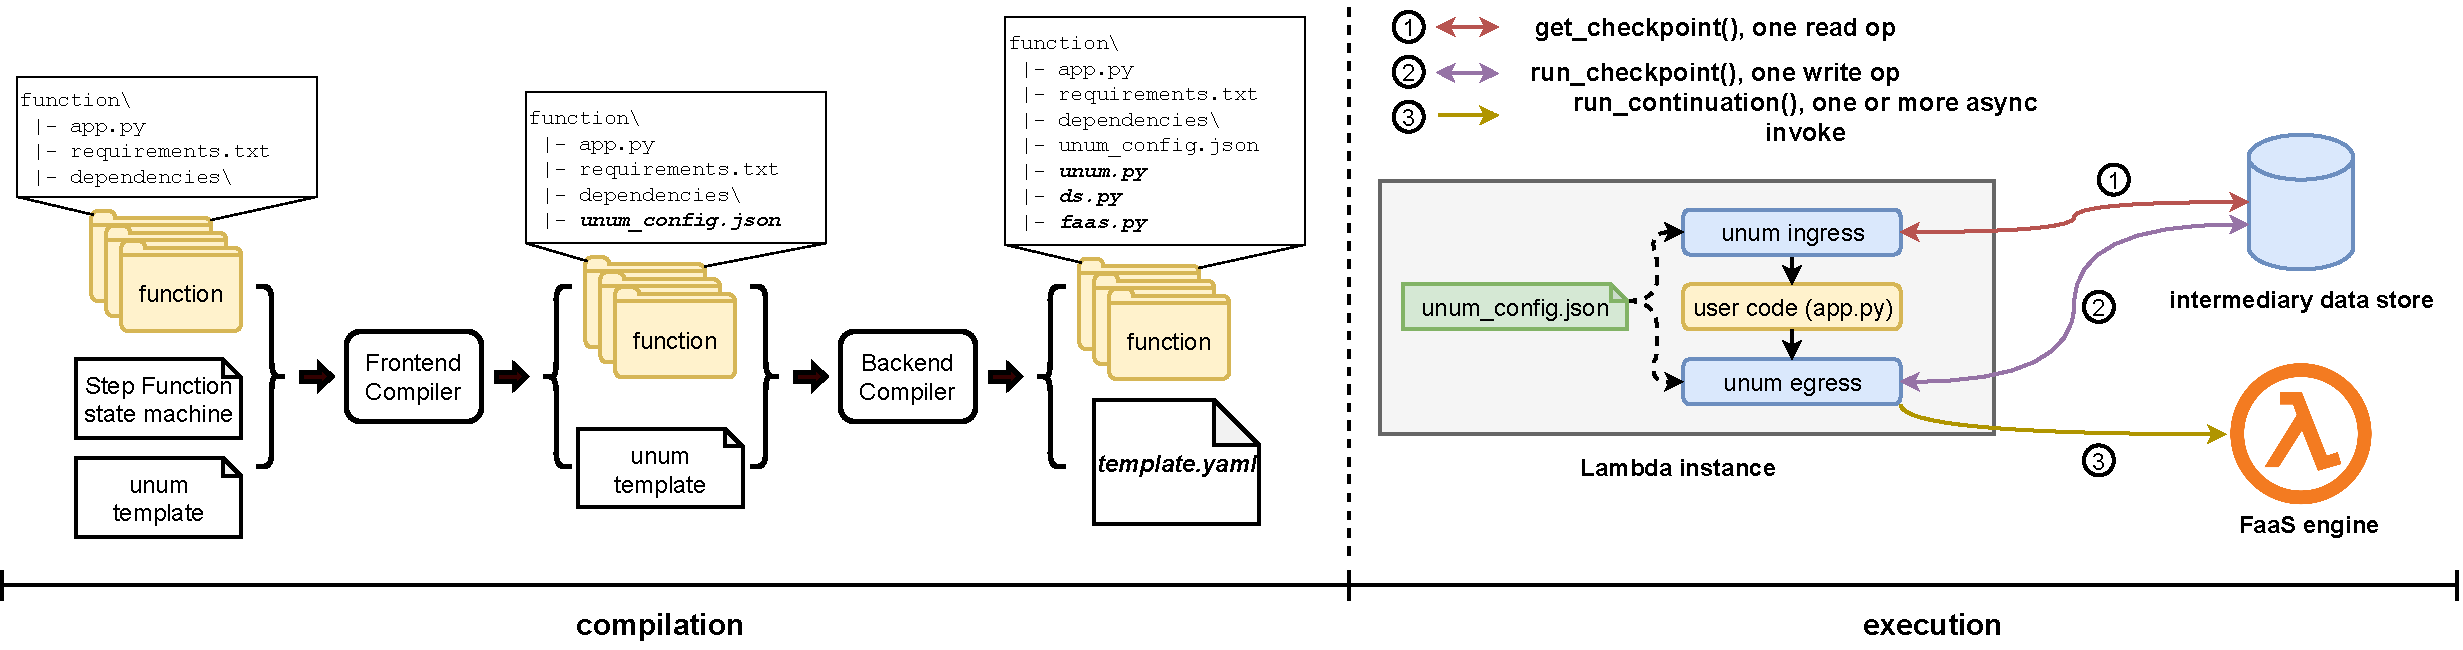
\includegraphics[width=\textwidth]{figures/unum-arch.pdf}
%    \caption{\name{}'s architecture}
%    \label{fig:arch}
%\end{figure*}

\begin{figure}[]
    \begin{minted}[
    frame=single,
    linenos,
    fontsize=\footnotesize
  ]{yaml}
Globals:
  ApplicationName: unum-iot-chain
  UnumIntermediaryDataStoreType: dynamodb
  UnumIntermediaryDataStoreName: iot-intermediary
  Checkpoint: true
  Debug: false
Functions:
  Aggregator:
    Properties:
      CodeUri: aggregator/
      Runtime: python3.8
      Start: true
  HvacController:
    Properties:
      CodeUri: hvac_controller/
      Runtime: python3.8
      Policies:
        - AmazonSQSFullAccess
  \end{minted}
    \caption{The unum template for an IoT HVAC controller
    application. It lists all resources of the workflow (Two functions:
    \texttt{Aggregator} and \texttt{HvacController}. A DynamoDB table
    \texttt{iot-intermediary} used as the intermediary data store) and
    specifies workflow-wide options such as checkpoint, debug and
    application name.}
    \label{fig:iot-unum-template}
\end{figure}


\begin{figure}[]
    \begin{minted}[
    frame=single,
    linenos,
    fontsize=\footnotesize
  ]{json}
{
  "StartAt": "Aggregator",
  "States": {
    "Aggregator": {
      "Type": "Task",
      "Resource": "Aggregator",
      "Next": "HvacController"
    },
    "HvacController": {
      "Type": "Task",
      "Resource": "HvacController",
      "End": true
    }
  }
}
    \end{minted}
    \caption{A Step Functions state machine for an IoT HVAC controller
    application. The workflow is a chain of two functions \texttt{Aggregator}
    and \texttt{HvacController}. When \texttt{Aggregator},
    \texttt{HvacController} should be invoked with \texttt{Aggregator}'s
    result. Note that normally the \texttt{"Resource"} fields are the deployed
    Lambda's ARN. Here they are function names defined in the unum template
    (see Figure~\ref{fig:iot-unum-template})}
    \label{fig:iot-sf}
\end{figure}

\begin{figure}[]
    \begin{minted}[
    frame=single,
    linenos,
    fontsize=\footnotesize
  ]{json}
{
    "Name": "string",
    "Next": {
        "Name": "FunctionName",
        "InputType": "Scalar" | "Map" | "Fan-in",
        "Condtional": "BooleanExpression"
    },
    "Next Payload Modifiers" : ["str"],
    "Checkpoint": "True | False",
    "Start": "True | False"
}
    \end{minted}
    \caption{}
    \label{fig:unum-config-lang}
\end{figure}

\begin{figure}[]
    \begin{minted}[
    frame=single,
    linenos,
    fontsize=\footnotesize
  ]{json}
{
    "Data": {
        "Source": "http | <data store type>",
        "Value": "<JSON object> | [<data store pointers>]"
    },
    "Session": "uuid",
	"Fan-out": {
        "Index": "int",
        "Size": "int",
        "OuterLoop": {
            "Index": "int",
            "Size": "int"
        }
    }
}
    \end{minted}
    \caption{}
    \label{fig:input-format}
\end{figure}

A key feature in \name{}'s approach is that it is designed as a runtime on top
of the serverless abstraction without requiring any supplemental services
added to current infrastructures. Workflows built with \name{} can execute in
any environment that has a FaaS engine with an asynchronous invocation API and
a named data store that supports strongly consistent reads. Both are readily
available on all existing serverless platforms.

Architecturally, \name{} eliminates the need for any specialized, hosted
processes that execute workflows, manage system states or broker
inter-function communication. FaaS functions are the only compute entity in
\name{} that runs code. They execute both user code and the \name{} runtime. The
\name{} runtime directly invokes the next function in the workflow after user
code completes and leverages a checkpointing mechanism to ensure strong
execution guarantees.

We continue this section by first giving an overview of unum's architecture
(\S~\ref{sec:design-overview}) and outlining the serverless abstractions and
services that \name{} builds upon (\S~\ref{sec:design-req}). We then
describe the programming interface that \name{} supports
(\S~\ref{sec:design-interface}). Next, we discuss the \name{} IR
(\S~\ref{sec:design-ir}) which expresses serverless workflows using
continuations. Finally, we describe \name{}'s runtime
(\S~\ref{sec:design-runtime}) and execution guarantees
(\S~\ref{sec:design-exec-gntee}).

\subsection{Overview}\label{sec:design-overview}

Figure~\ref{fig:arch} illustrates \name{}'s high-level architecture. At
compile-time, a frontend compiler transforms workflows written for existing
systems (e.g., an AWS Step Functions state machine that orchestrates Lambdas)
into a continuation-based, platform-independent intermediary representation.
In practice, the IR is a set of configuration files
(\texttt{unum\_config.json}), one for each function in the workflow, written
in the \name{} configuration language (\S~\ref{sec:design-config-lang}).

Next, a backend compiler compiles the IR into platform-specific packages that
are executable in a particular target environment (e.g., AWS Lambda with
DynamoDB as the data store). Deploying the packages will create a set of FaaS
functions (e.g., Lambdas) and an intermediary data store (e.g., a DynamoDB
table or S3 bucket).

A workflow is invoked by triggering the entry function. Each unum workflow has
one and only one entry function. \shadi{does it have to be one entry point? why?}

At execution time, each function runs both the user code and the unum runtime.
The unum runtime manages the function's checkpoint and invokes the
continuation asynchronously after user code completes. unum uses checkpoints
to provide strong execution guarantee. Every function invocation in unum is
assigned a unique name and the runtime uses the name for the instance's
checkpoint in the data store.

\subsection{System Requirements}\label{sec:design-req}

\name{} utilizes two services that are readily available on all existing
serverless platforms:

\begin{enumerate}

	\item A Function-as-a-Service engine that supports an
	\emph{asynchronous invocation API}.

	\item A shared data store that supports creating and reading items by
	 their unique names.

\end{enumerate}

\subsubsection{FaaS engine with asynchronous invocation}

Support for asynchronous invocation is universal across all major FaaS
engines, including AWS Lambda~\cite{aws-lambda-async-invoke}, Azure
Functions~\cite{azure-functions-async-invoke}, Google Cloud
Functions~\cite{google-cloud-functions-async-invoke}, and popular open-source
options such as OpenWhisk~\cite{openwhisk-async-invoke} and
OpenFaaS~\cite{openfaas-async-invoke}.

\name{} chooses asynchronous invocation because functions in \name{} directly invoke
their immediate downstream functions and asychronous invocation avoids
timeouts, and double billing. If only synchronous invocation is available, a
function has to idly wait for all of its downstream functions, immediate or
not, to complete, risking function timeouts and incurring double billing.

\paragraph{At-least-once invocation}

FaaS engines normally only guarantee at-least-once invocation of
asynchronously triggered
functions~\cite{google-cloud-functions-exec-guarantee,
aws-lambda-async-invoke, azure-functions-exec-guarantee}. A single invocation
might result in the FaaS engine running the same function more than once. Such
duplicate invocations are especially problematic when the function is
non-deterministic (i.e., given the same input, the function might produce
different output across runs) and all serverless providers simply urge
developers to write deterministic functions to avoid incorrect behavior.

From a workflow system's perspective, it has a few options to work with an
at-least-once FaaS engine: (1). it can equire all functions to be
deterministic (2). make sure functions are invoked exactly-once (3). ensure
that even if a non-deterministic function executes more than once, only one of
the results is taken as the final result and propagated to the rest of the
workflow.

\name{} takes the third approach as the first is restrictive and the second is
unattainable. \name{} uses a checkpointing mechanism to make sure only the
execution that finishes first is taken as the final result and propagated
downstream. Duplicates are simply discarded. We discuss the details in
\S~\ref{sec:design-runtime}.

\subsubsection{Named data store}

Functions in \name{} workflows use a named data store to store checkpoints and
other intermediary data (\S~\ref{sec:design-runtime}) during execution. The
data store needs to support creating and later retrieving objects with unique
names.

There is a wide variety of data store services that can support \name{}
workflows, including object storage (e.g., Amazon S3, AZure Blob Storage),
NoSQL databases (e.g., DynamoDB, Cosmos DB) and key-value stores (e.g.,
Redis).

Nearly all of the storage services above have a "serverless" option that
requires no explicit provisioning and users only pay for what they use.

\paragraph{Consistency Requirements}

\name{} requires the data store to be strongly consistent.

Strongly consistent reads (read that return the most up-to-date data,
reflecting all prior writes that were successful) are important for the
correctness of aggregations (e.g., fan-in), because it prevents the
possibility where all upstream functions have completed and written their
checkpoint but none of them sees that all have completed and thus never invoke
the fan-in function.

Note that strong consistency alone is not enough for correct execution of
aggregation patterns because multiple functions might detect that all fan-out
branches have completed and thus invoking the fan-in functions more than once.
\name{} runtime contains additional synchronization logic to make sure the fan-in
function is only invoked once. We discuss the details in
\S~\ref{sec:design-runtime}


\subsection{Programming Interface}\label{sec:design-interface}

\name{} does not introduce a new programming interface for building serverless
workflows. Developers can use familiar frontend languages from existing
systems, such as the Amazon State Language for AWS Step Functions.

Moreover, \name{} lets developers write component functions in
workflows exactly the same way as they would for regular functions. In fact,
orchestration-related logic are entirely transparent from user functions'
perspective. There is no additional libraries that user code needs to import
or use.

Figure~\ref{fig:arch} gives an example of using Step Functions state machine
to define the workflow that orchestrates functions in Python. Each
function is defined in its own directory with the exact same content as you
would have for regular functions that are not part of any workflow.

The \emph{unum template} is a YAML file that lists all the resources in the
workflow and specifies workflow-wide configurations.
Figure~\ref{fig:iot-unum-template} gives an example of an IoT HVAC controller
application's template.

The frontend compiler transforms the workflow definition to a
continuation-based, platform-independent intermediary representation (IR)
which we discuss in the next section.



\subsection{\name{} IR}\label{sec:design-ir}

The \name{} intermediary representation expresses FaaS workflows using
continuations. A continuation defines (1). which function(s) to invoke (2).
what input to invoke it with.

After running user code, the unum runtime invokes the continuation with the
user code's result as the input. Every function in a unum workflow has 0, 1 or
more continuations. The set of continuations from all functions form the
complete workflow.

unum continuations form graphs with functions as vertices. They support common
orchestration patterns such as chaining, branching, fan-out and fan-in. unum
also supports \texttt{for} or \texttt{while} loop (fold) with continuation
graphs that have directed cycles.

A key benefit of the continuation-based IR is to distribute workflows'
orchestration logic to individual component functions so that it can execute
without a centralized orchestrator. In an orchestrator-based workflow system,
functions will need to call back to the orchestrator service to signal
completion and it is the orchestrator who will then invoke the next function.

In contrast, unum assigns each function a set of continuations \emph{at
compile-time}. After user code completes, each function directly invokes its
continuations asynchronously, without involving any supplemental services.

% \subsubsection{Naming scheme}

% \name{} assigns each function instance a unique name. The name consists of the
% function's name and, if the instance is part of a fan-out, the instance's
% fan-out index.



\subsubsection{\name{} configuration language}\label{sec:design-config-lang}

In practice, the \name{} IR is a set of configuration files (by default named
\texttt{unum\_config.json}), one for each function in the workflow, written in
the \name{} configuration language.

Figure~\ref{fig:patterns} shows 2 examples patterns and how to express them in
the \name{} IR.

The configuration language provides constructs to define continuations. Each
continuation is a JSON object. It specifies the name of the function to invoke
(the \texttt{"Name"} field), what its inputs are (the \texttt{"InputType"}
field) and an invoke condition (the \texttt{"Conditional"} field).

The function name needs to match one of the names in the \name{} template. The 

Continuations are defined in the \texttt{"Next"} field. The value is
either a single JSON object if there is only one continuation or an array
of JSON objects if there are multiple continuations.

% Figure~\ref{fig:iot-sf} shows a Step Functions state machine for an IoT HVAC
% controller workflow which is a chain of two functions. Figure~\ref{fig:iot-ir}
% shows the generated IR in the form of two \texttt{unum\_config.json} files.

\begin{itemize}

	\item Every function has a \texttt{unum\_config.json} file deployed with
	it.

	\item Continuations are defined in the \texttt{"Next"} field. The value is
	either a single JSON object if there is only one continuation or an array
	of JSON objects if there are multiple continuations.

	\item Each continuation is a JSON object. It specifies the name of the
	function to invoke next in the \texttt{"Name"} field, what its inputs are
	in the \texttt{"InputType"} field and an invoke condition in the
	"Conditional" field.

	\item \texttt{"InputType"} has three possible values: \texttt{"Scalar"},
	\texttt{"Map"} and \texttt{"Fan-in"}.

	\item \texttt{"Scalar"} is used when the only input to the next function
	is the output of this function.

	\item \texttt{"Scalar"} supports chaining, where the input to the next
	function is the output of the previous function, and fan-out, where
	multiple functions are triggered in parallel with the output of the
	previous function.

	\item Give example \texttt{unum\_config.json} files of chaining and
	fan-out with \texttt{"Scalar"}?

	\item \texttt{"Map"} supports a different form of fan-out where the output
	of this function is an array and for each element of the array, the
	runtime invokes one instance of the next function with the element as
	input.

	\item \texttt{"Fan-in"} is used for aggregations when the next function to
	invoke depends not only on the result of this function but also on those
	of other functions. (Give a concrete example here?)

	\item Values that the next function depends on are listed in the
	\texttt{"Values"} field. Each value is identified by the unique name of
	the function instance that produces it. We discuss \name{}'s naming scheme
	in the next section.

	\item Value names can include glob patterns to support fan-in of varying
	size. unum expands glob patterns during runtime.

	\item The "Conditional" field is a boolean expression. Only when the
	boolean expression evaluate to Ture would the continuation be invoked.

	\item Workflow entry functions have \texttt{"Start: true"}.

	\item "Next Payload Modifiers" is an interface to modify \name{}'s runtime
	metadata. 

\end{itemize}


\subsection{Runtime}\label{sec:design-runtime}

\begin{itemize}

	\item \name{}'s runtime interposes on user code's entry and exit (See
	Figure~\ref{fig:arch}. On ingress, \name{} runtime reads the input data
	and then pass it to user code. When user code returns, the egress takes
	the return value, write it to the data store as a checkpoint and invokes
	the continuation.

	\item Inputs to unum functions are JSON objects.
	Figure~\ref{fig:input-format} shows the input format.

	\item \texttt{"Data"} field contains the input data to the user code. If
	the data is directly sent in the function invocation via HTTP (i.e.,
	\texttt{"Source": "http"}), the value of the "Value" field is passed to
	user code unchanged. If the \texttt{"Source"} field shows that the data is
	in the intermediary data store (e.g., \texttt{"Source": "dynamodb"}),
	\name{} reads the data from the data store and then pass it to user code.

	\item In practice, \name{} only passes data via the data store in the case
	of fan-in where results of multiple functions are needed. In that case,
	the \texttt{"Value"} field is an array of names of function checkpoints.
	\name{} reads each checkpoint in the array in order and passes the data as
	an array to user code.

	\item User code is oblivious of the \name{} runtime. \name{} does not
	change how user code is written or its interface.

	\item \texttt{"Session"} field contains a UUID string that uniquely
	identifies a workflow invocation. \name{} runtime on the entry function
	creates the UUID string when the function is invoked. The string
	propagates to all downstreams function instances that are part of the
	workflow invocation.

	\item Checkpoint names are prefixed with the \texttt{"Session"} UUID
	string so that instances of the same function from different invocations
	do not overwrite each others' results.

	\item "Fan-out" field are part of fan-out functions' input payload.
	\name{} assigns each fan-out function an index.

	\item \name{} supports nested fan-outs with the \texttt{"OuterLoop"} field
	that is recursive.

	\item Each function instance is assigned a unique name. The name consists
	of the function's name and, if the function is part of a fan-out, its
	fan-out indexes. Example?

	\item Fan-in semantics. Only invoke the continuation once when all inputs
	are ready. For data stores with atomic data structures, we use them to
	synchronize. For data stores without atomic data structures, \name{}
	pre-select that last function in the \texttt{"Value"} array to wait for
	all other functions to complete.

\end{itemize}

% \subsubsection{Checkpoints?}


% check checkpoint existence before running user function

% run user function or read from existing checkpoint

% write checkpoint or pass

% run continuation

% checkpoints are used both for guaranting execution correctness and for
% aggregation patterns such as fan-in.


\subsection{Fault tolerance and execution guarantee}\label{sec:design-exec-gntee}

Challenges to providing strong execution guarantees:

\begin{enumerate}

	\item Functions in the workflow can fail at any point.

	\item FaaS engines only provide at-least-once execution guarantee on
	individual functions. Triggering a function once might result in duplicate
	executions.

\end{enumerate}

Given the limitation of the underlying FaaS engines, \name{} cannot guarantee
exactly-once execution on \emph{individual functions}. However, \name{}
guarantees:

\begin{enumerate}

	\item At-least-once invocation on individual functions. This ensures that a
	workflow invocation will not just stuck somewhere and not proceed.

	\item In a particular workflow invocation, a particular function will
	always be invoked with the exact same input.

	\item Each workflow invocation will produce exactly one result. Even if
	there happen to be duplicate executions of functions, and even if the
	functions are non-deterministic, only a single result is recorded, while
	any duplicate and potentially diverging results are discarded.

\end{enumerate}

From users' perspective, if none of the functions in the workflow have
external side-effects (e.g., writing to external services), the workflow will
appear to execute exactly-once.

\name{} leverages the at-least-once execution guarantee of FaaS engines to
ensure that functions run at least once.

When a workflow execution crashes before finishing, \name{} only retries the
function where the crash happens instead of restarting the entire workflow.
\name{} leverages the automatic retry feature that most FaaS engines already provide
for individual functions~\cite{azure-functions-retry,
google-cloud-functions-retry, aws-lambda-async-invoke}.

\name{} uses checkpointing to make sure that even if a function executes more
than once, whether due to retries or duplicate invocations, only the result of
one of the executions is taken as the final result, and only the final result
is propagated downstream to the rest of the workflow.

\name{} checkpointing process is the following:

First, before running user code, the ingress checks to see if a checkpoint
already exists for the invocation. If it does, \name{} skips running user code
and uses the checkpoint's content as the result. The egress will invoke the
continuation again in case the prior execution crashed after checkpointing but
before running the continuation. This makes sure that if a step in the
workflow has completed and persisted, it will not run again.

If a checkpoint doesn't exist, unum runs the user code. After the user
function completes, unum checkpoints the result into the data store and runs
the continuation.
